\begin{defnbox}\nospacing
    \begin{defn}[Symbolic Tracing]\label{defn:symbolic_tracing}\leavevmode\\
        \begin{minipage}[c]{0.52\textwidth}
            Is the capture and representation of python operations as a symbolic graph.
        \end{minipage}\hfil
        \begin{minipage}{0.4\textwidth}
            \begin{figure}[H]
                \centering
                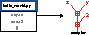
\includegraphics[width=0.9\textwidth]{pytorch_submodule/src/the_framework/graph_acquisition/figures/code_to_graph.pdf}
            \end{figure}
        \end{minipage}
    \end{defn}
\end{defnbox}

\begin{defnbox}\nospacing
    \begin{defn}[Computation Graph]\label{defn:computation_graph}\leavevmode\\
        A computation graph is a representation that can tracks data flow and operations and that can be used for automatic differentiation.
    \end{defn}
\end{defnbox}
\begin{defnbox}\nospacing
    \begin{defn}[Dynamic Graph Computation]\label{defn:dynamic_graph_computation}\leavevmode\\
        A dynamic graph is a graph that tracks operations and data flow dynamically during the execution of the code.
    \end{defn}
\end{defnbox}


%%% Local Variables:
%%% mode: latex
%%% TeX-command-extra-options: "-shell-escape"
%%% TeX-master: "../../../../formulary"
%%% End:
